\problemname{Light Bulbs}

Shortly after founding his lightbulb company in Eindhoven in 1891, Frederik Philips made a great discovery: lightbulbs
that light up an infinite ray in the horizontal or vertical direction. With this new discovery, he
wants to revolutionize the interior design of modern homes.

He plans an elaborate installation with his son, Gerard. They install $N^2$ lamps in an $N \times N$
grid in a room.
They want to light up the whole room with as few lamps turned on as possible to save electricity.
Each lamp is either vertical, meaning it lights up all squares in its column, or horizontal, meaning it lights up all squares in its row.

The illustration below shows an example of a vertical (left) and a horizontal (right) lamp.

\begin{figure}
\centering
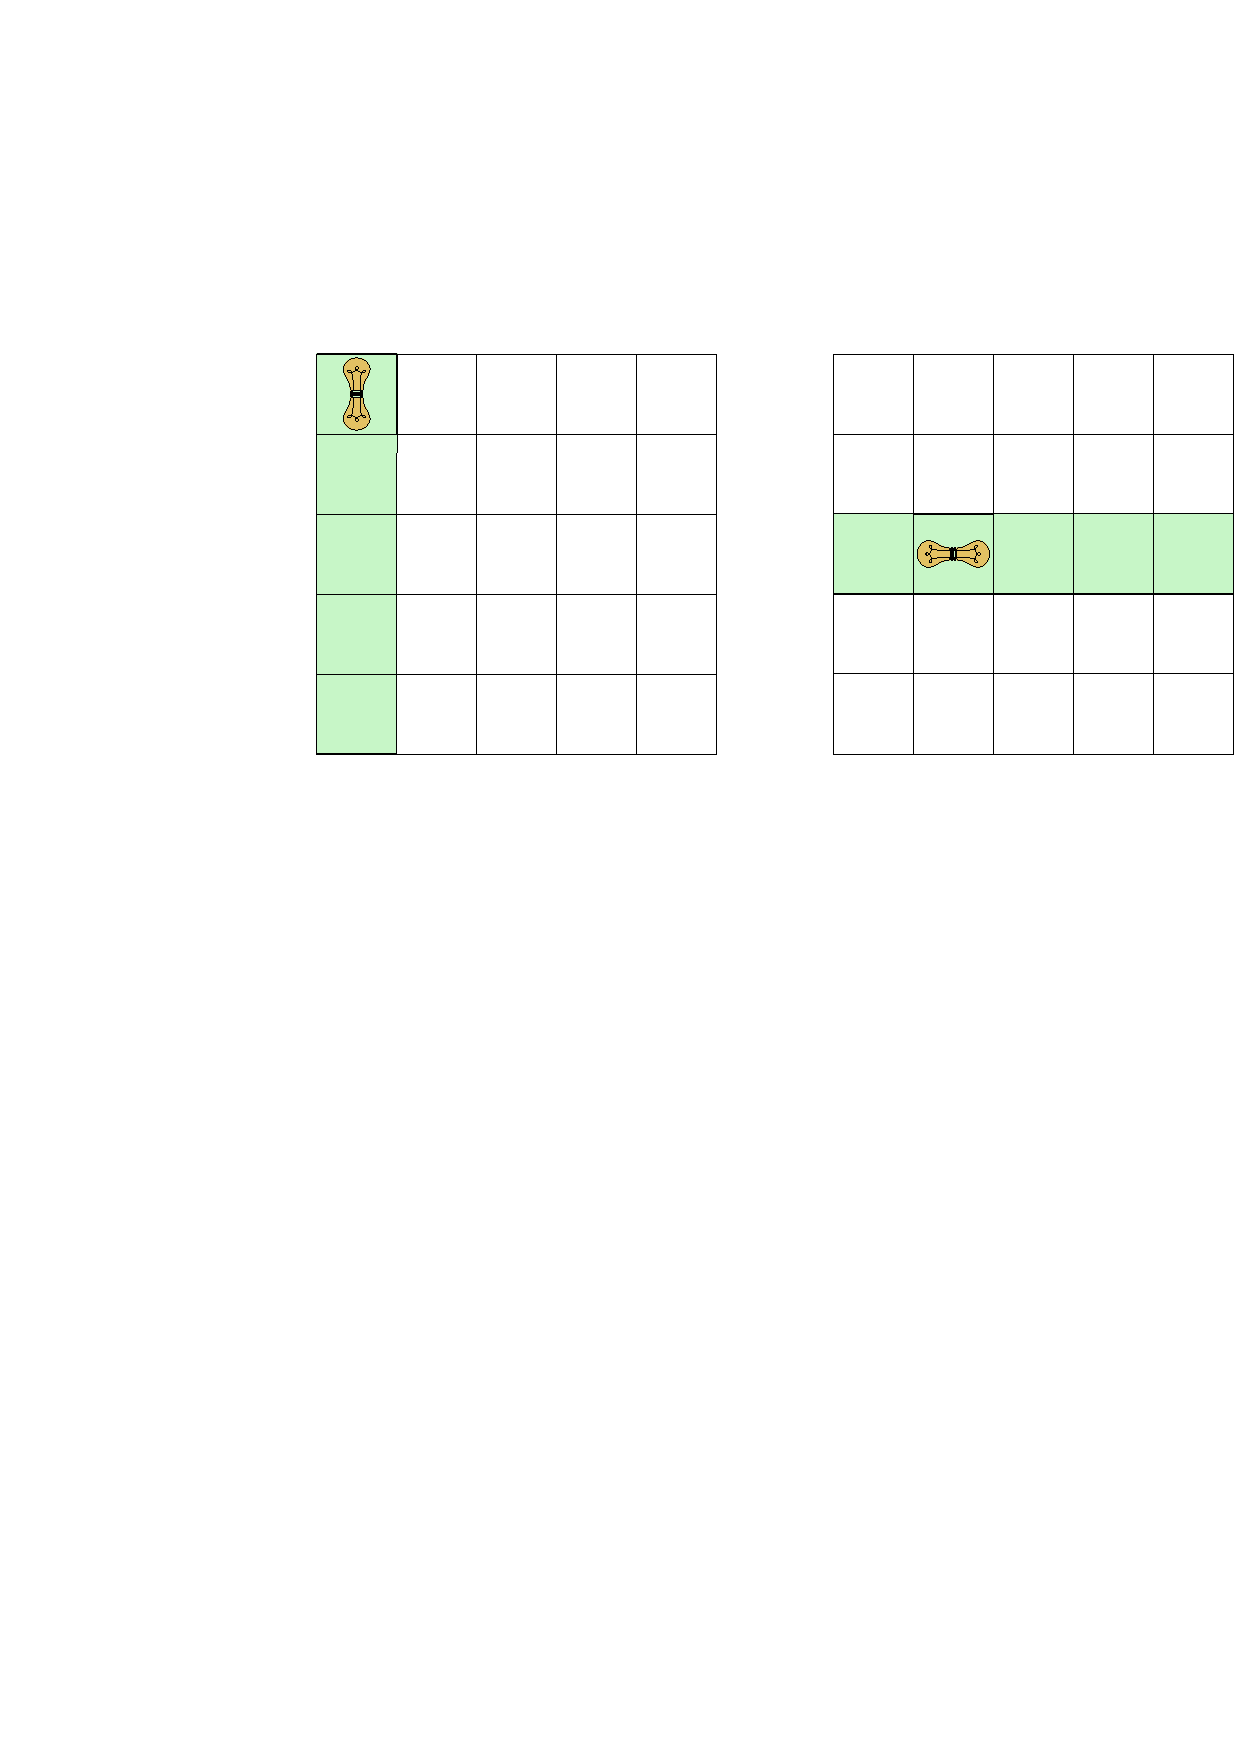
\includegraphics[width=0.7\textwidth]{vert_horiz.pdf}
\end{figure}

Unfortunately, they did not pay attention when installing
the lamps and do not remember which lamps light up horizontally or vertically.
Instead, they conduct some experiments to figure out which lamps to use to light up the whole room.
Gerard stays in the room with the lamps, while Frederik operates the switches from another room.

In each experiment, Frederik turns each lamp on or off and Gerard reports how many squares are lit up in total; a square that is lit up by two or more separate lamps is only counted once.
It does not matter how many lamps are turned on during the experiments, but they are in a rush and ideally want to conduct as few experiments as possible.

Help them find an arrangement of lamps that lights up the whole room and uses the fewest lamps. They can conduct at most $2\,000$ experiments. However, you will get a higher score if they use fewer experiments.

\section*{Interaction}
This is an interactive problem.

\begin{itemize}
\item Your program should start by reading a line with an integer $N$, the height and width of the grid.
\item Then, your program should interact with the grader.
    To conduct an experiment, you should first print a line with a question mark ``\texttt{?}''.
On the next $N$ lines, output an $N \times N$ grid specifying which lamps are lit.
Specifically, on each of these lines, output a string of length $N$, consisting of $0$'s (turned off) and $1$'s (turned on).
Then, your program should read a single integer $\ell$ ($0 \leq \ell \leq N^2$), the number of grid squares lit up by turning on the lamps specified.
\item When you want to answer, print a line with an exclamation mark ``\texttt{!}'', followed by $N$ lines with the grid in the same format as above.
In order for your answer to be accepted, the \textbf{lamps must light up the whole grid and the number of turned-on lamps must be the fewest possible}.
\end{itemize}

After this, your program should exit.

The grader is non-adaptive, meaning that the grid of lamps is determined before the interaction begins.

Make sure to flush standard output after issuing each experiment; otherwise, your program might get judged as ``Time Limit Exceeded''.
In Python, this happens automatically as long as you use \texttt{input()} to read lines. In C++, \texttt{cout << endl;} flushes in addition to printing a newline; if using \texttt{printf}, use \texttt{fflush(stdout)}.

\section*{Constraints and Scoring}
\begin{itemize}
\item $3 \le N \le 100$.
\item You can issue at most $2\,000$ experiments (printing the final answer does not count as an experiment). If you exceed this, you will get the verdict ``Wrong Answer''.
\end{itemize}


Your solution will be tested on a set of test groups, each worth a number of points.
Each test group contains a set of test cases. To get the points for a test group, you need to solve all test cases in the test group.

\begin{tabular}{|l|l|l|}
\hline
Group  &  Score  &  Limits \\
\hline
 1 & 11 & $N = 3$  \\
\hline
 2 & 11 & $N\le 10$ \\
\hline
 3 & up to 78 & No additional constraints \\
\hline
\end{tabular}


In the final test group, your \textbf{score depends on the number of experiments you conduct}, calculated by the following formula:

$\text{score} = \begin{cases}
  (2000-Q)\cdot 29/ 900& \text{if } 200 \le Q \le 2000, \\\
  58 + (200-Q)\cdot 4 / 23 & \text{if } 85 \le Q \le 200, \\\
  78 & \text{if } Q \le 85,
\end{cases}$

where $Q$ is the maximum number of experiments used on any test case.
The score will be rounded down to the nearest integer.

The plot below shows the number of points, as a function of $Q$, your program will get if it solves all test groups.
To obtain a full score of 100 points on this problem, you must solve each test case using at most 85 experiments.


\begin{figure}
\centering
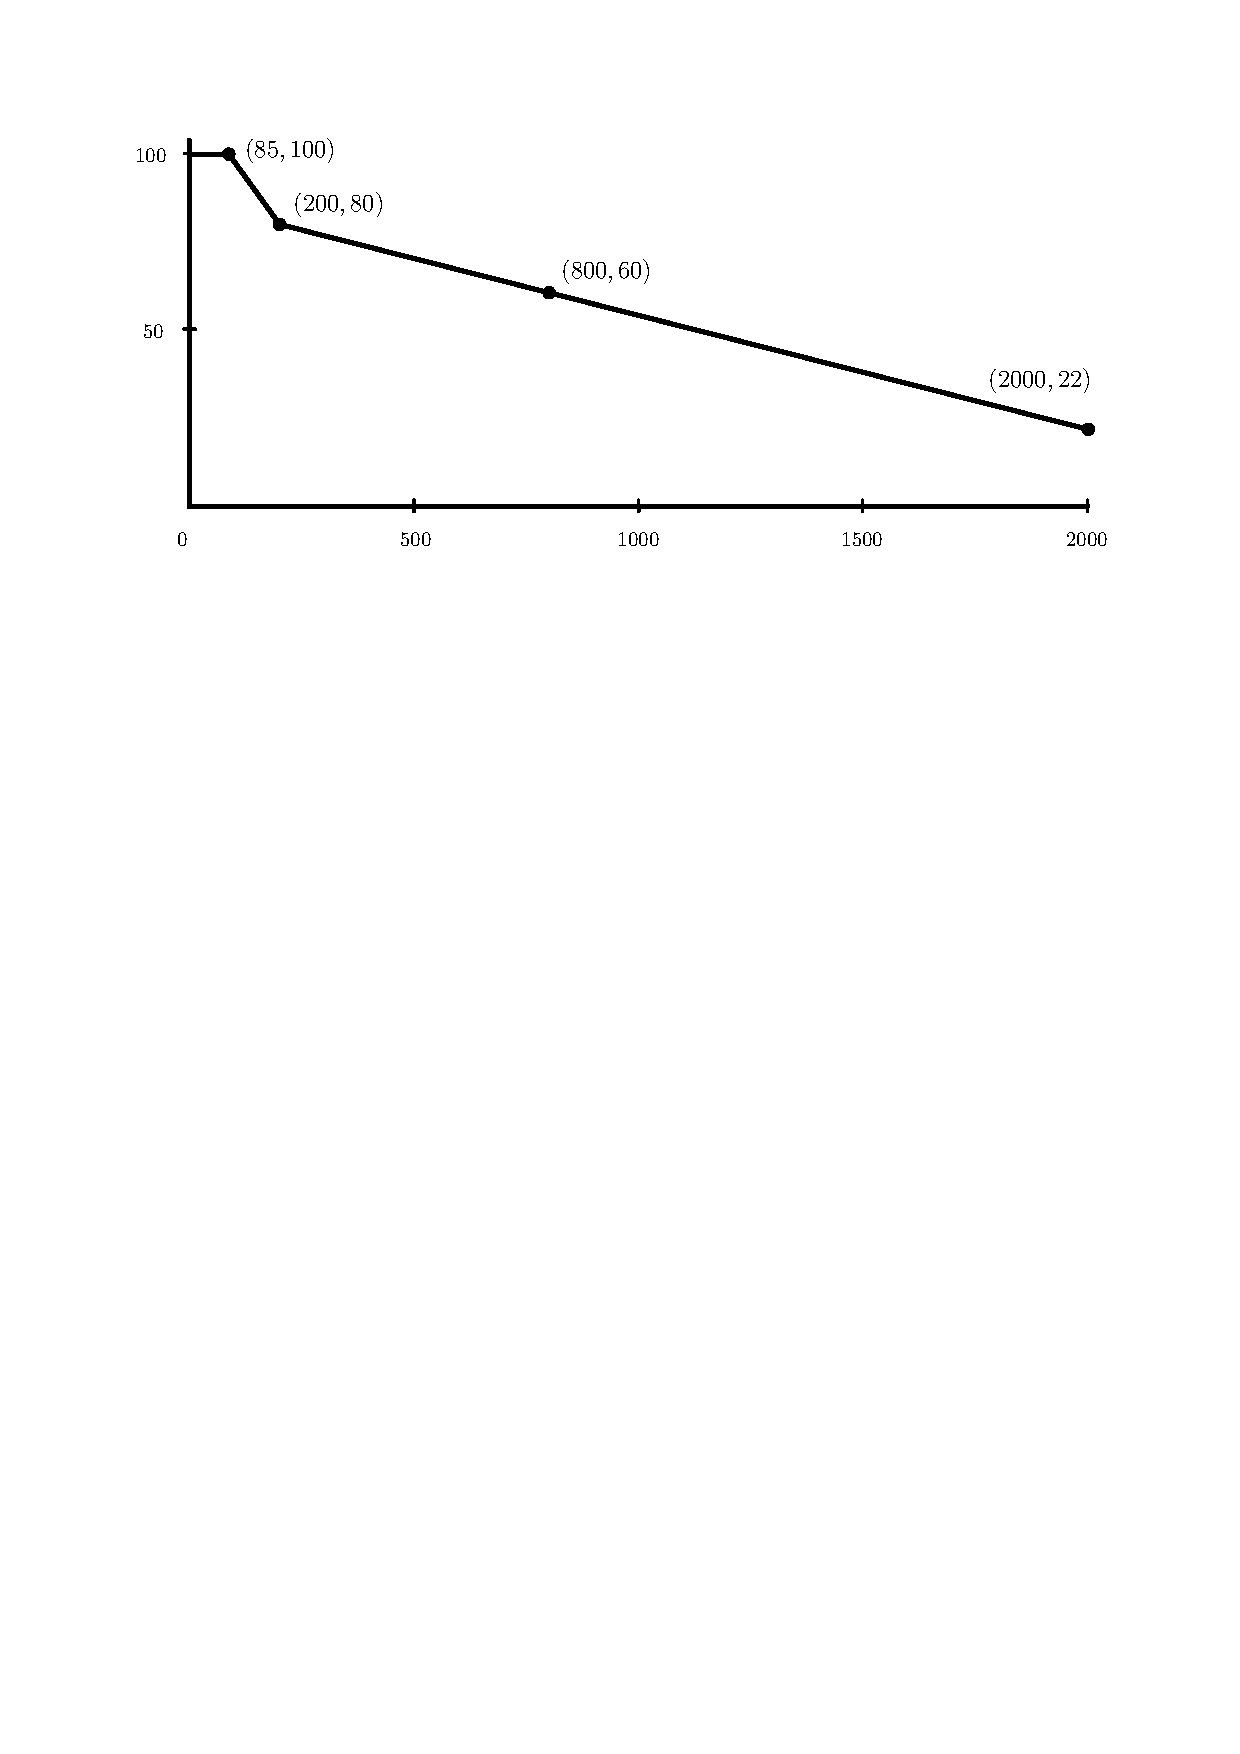
\includegraphics[width=0.7\textwidth]{scoreplot.pdf}
\end{figure}

\section*{Testing Tool}
To facilitate the testing of your solution, we provide a simple tool that you can download.
See ``attachments'' at the bottom of the Kattis problem page. The tool is optional to use. Note that the official grader program on Kattis is different from the testing tool.

To use the tool, create an input file, such as ``sample1.in'', which should start with a number $N$ followed by $N$ lines specifying the grid, where \texttt{V} means that the lamp lights up its column and \texttt{H} means that it lights up its row. For example:

\begin{verbatim}
  5
  VVHVH
  HVHHV
  VHHVV
  HHHVH
  HHVVV
  \end{verbatim}


  For Python programs, say \verb|solution.py| (normally run as \verb|pypy3 solution.py|):

  \verb|python3 testing_tool.py pypy3 solution.py < sample1.in|

\noindent
For C++ programs, first compile it
(e.g. with \verb|g++ -g -O2 -std=gnu++20 -static solution.cpp -o solution.out|)
and then run:

  \verb|python3 testing_tool.py ./solution.out < sample1.in|

\section*{Example}
In the sample interaction, the program starts by reading the grid size $N = 5$.
The following figure shows the hidden grid (which the program does not know) and one of many potential answers, using five lamps to light up the whole grid.
The marked lamps are turned on and the darker squares are lit up.

\begin{figure}
\centering
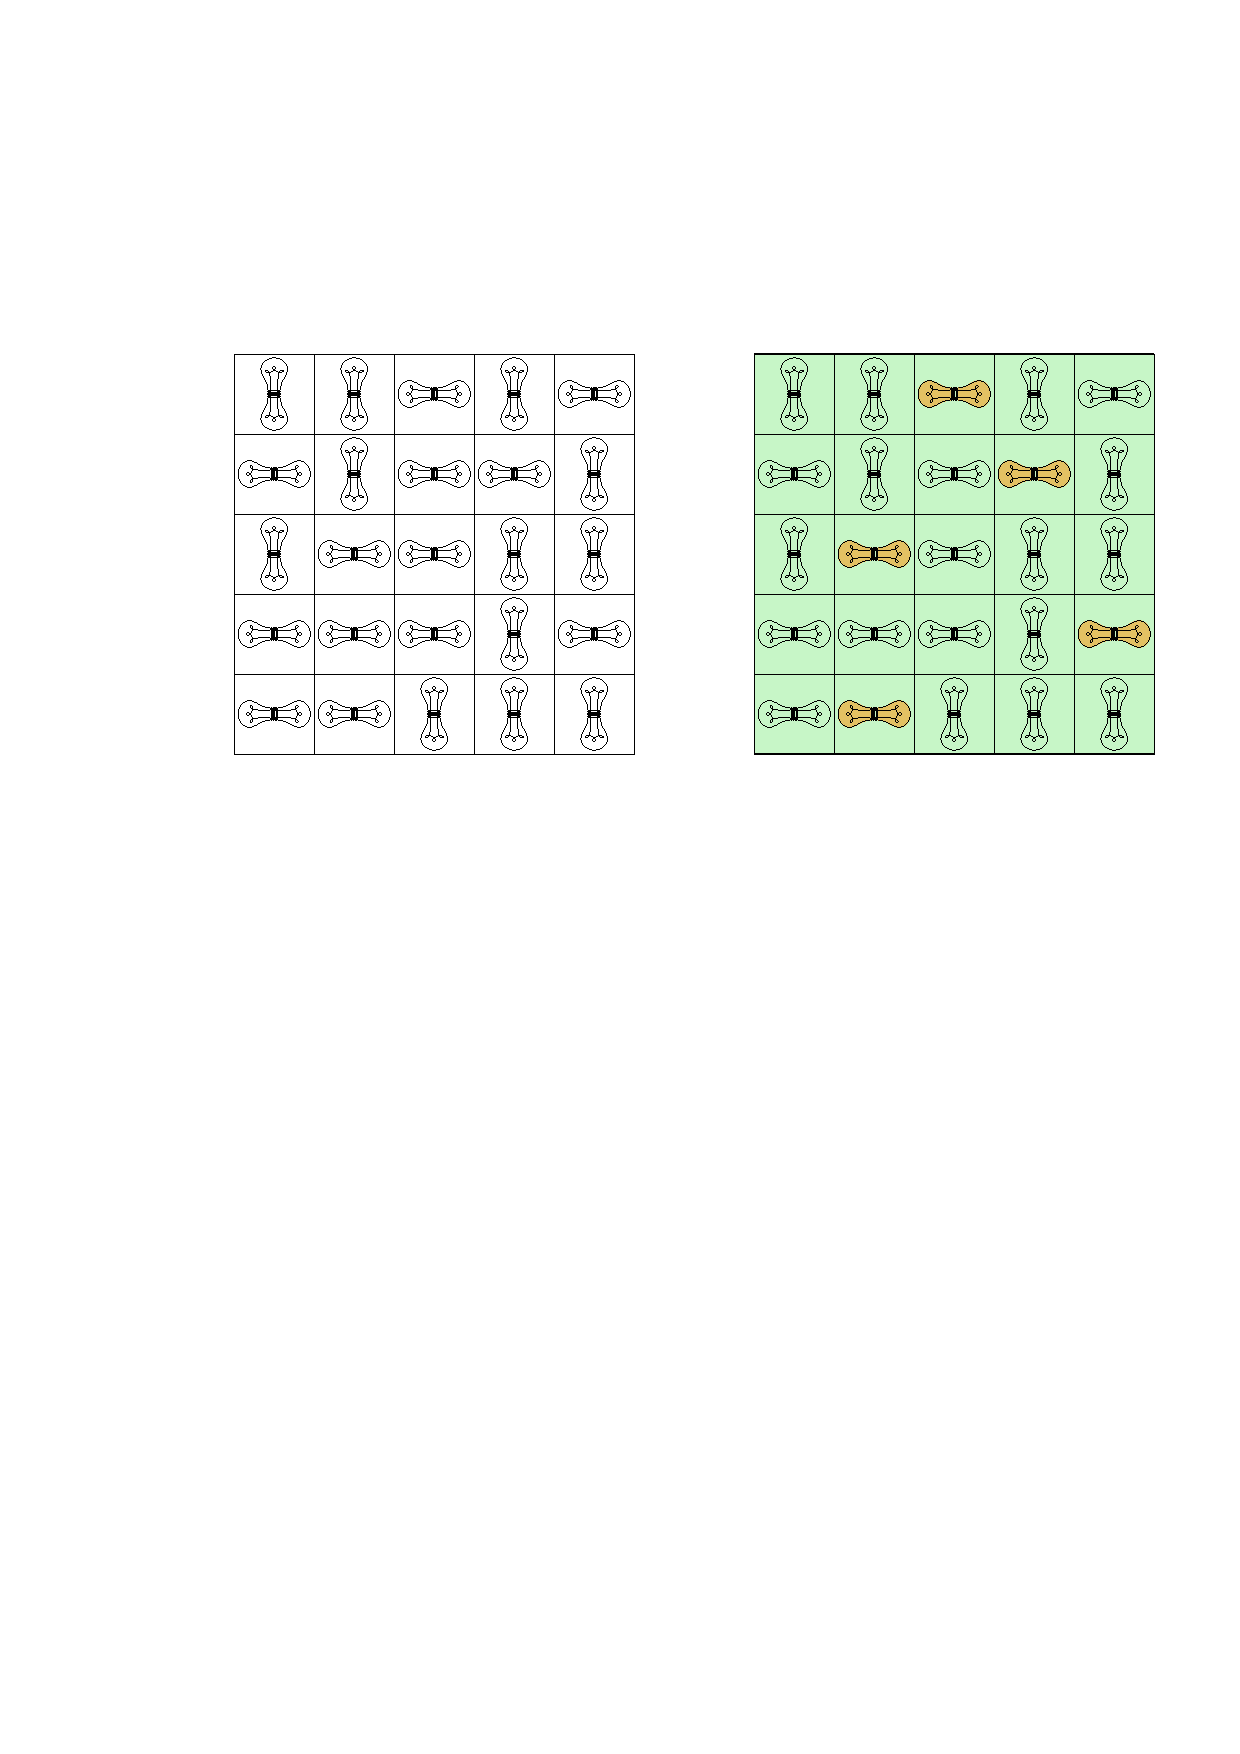
\includegraphics[width=0.9\textwidth]{fig1_4.pdf}
\end{figure}

The program performs two experiments as illustrated below. In the first
   experiment, a total of 10 squares are lit up using the two vertical lamps in the top left corner.
 The second experiment lights up a total of 13 squares.
 Finally, the program writes its answer (illustrated above) and exits.

\begin{figure}
\centering
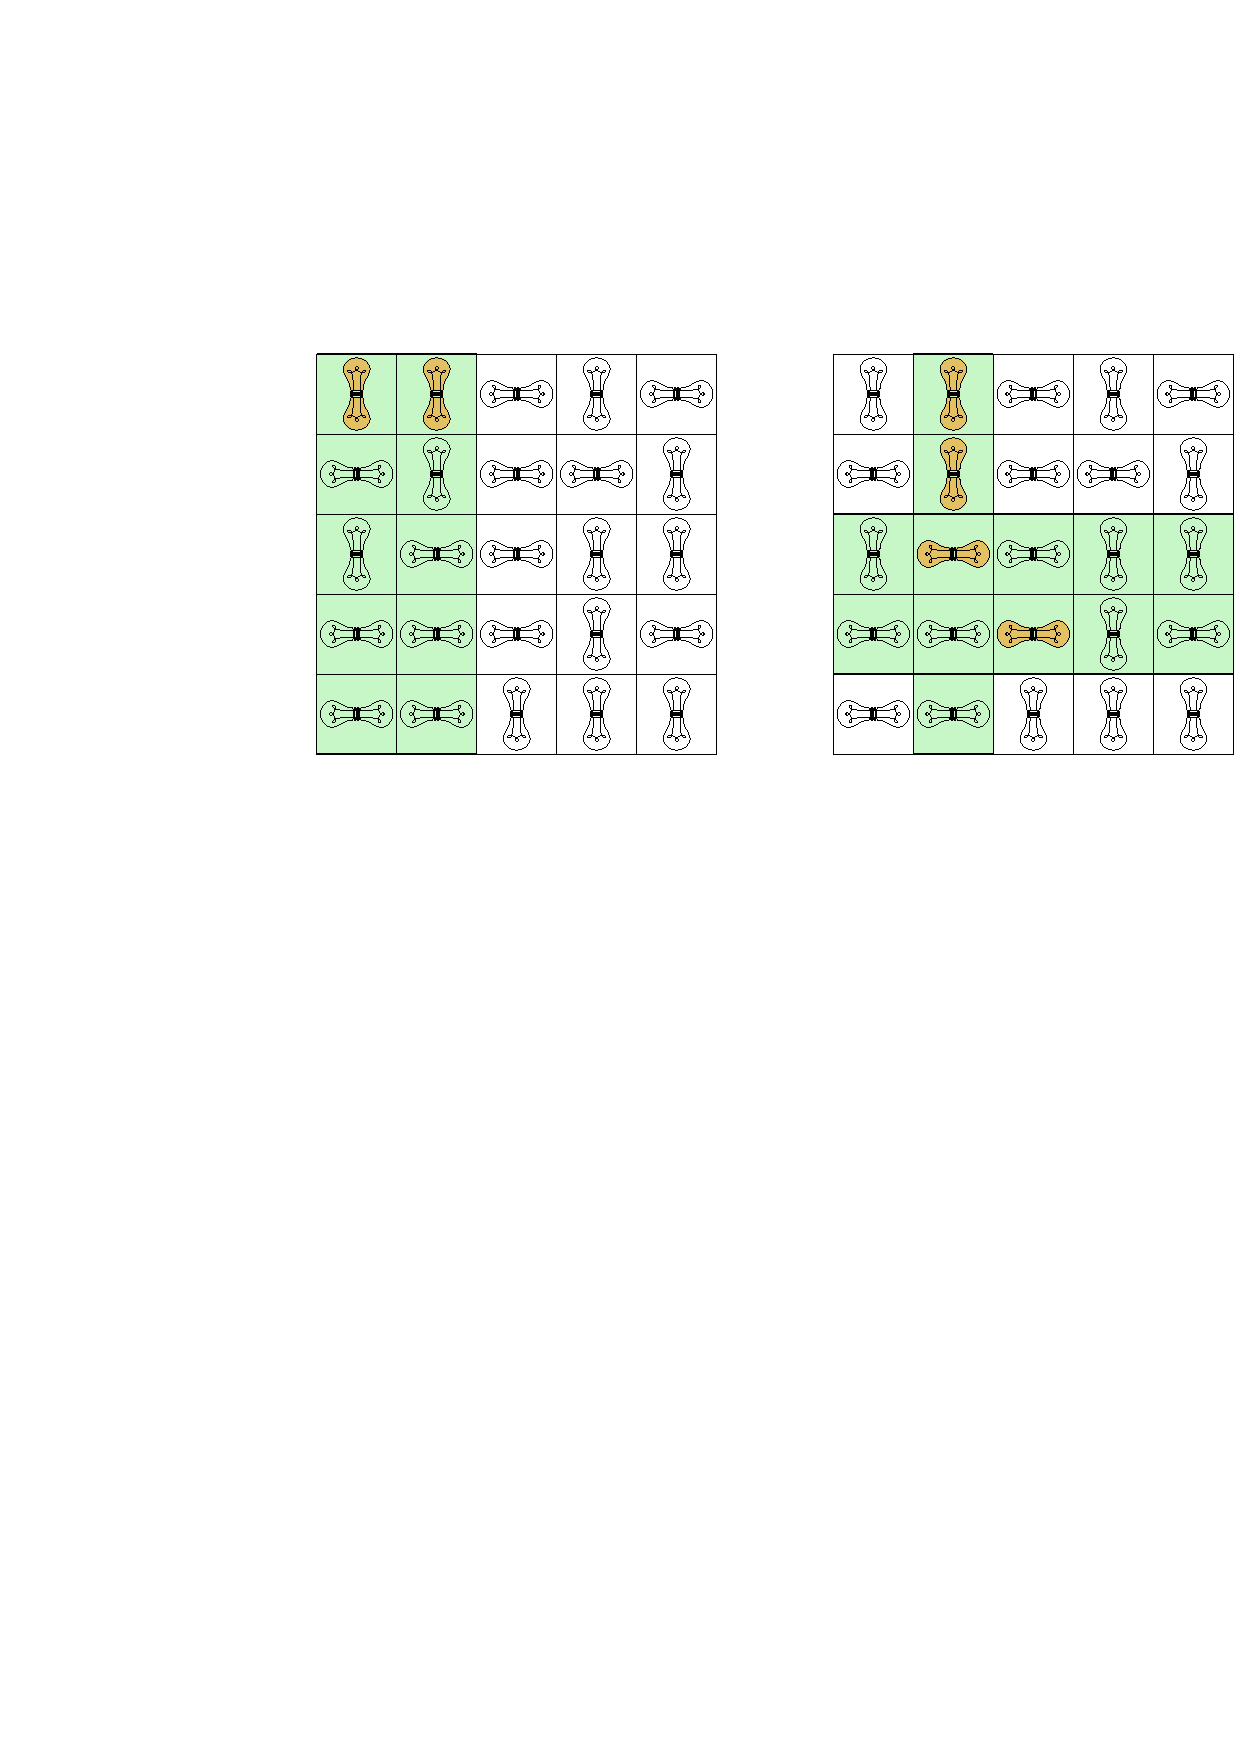
\includegraphics[width=0.9\textwidth]{fig2_3.pdf}
\end{figure}
